%%%%%%%%%%%%%%%%%%%%%%%%%%%%%%%%%%%%%%%%%
% Medium Length Graduate Curriculum Vitae
% Downloaded from http://www.LaTeXTemplates.com
% Courtesy of Rensselaer Polytechnic Institute (http://www.rpi.edu/dept/arc/training/latex/resumes/)
%%%%%%%%%%%%%%%%%%%%%%%%%%%%%%%%%%%%%%%%%

\documentclass[margin, 10pt]{Stylesheet}

\usepackage{helvet}
\usepackage{hyperref}
\usepackage{textcomp}
\usepackage{graphicx}
\usepackage{setspace}
\setlength{\textwidth}{5.1in}

\begin{document}

\noindent\begin{minipage}{0.4\textwidth}% adapt widths of minipages to your needs
\hspace*{-1.2cm}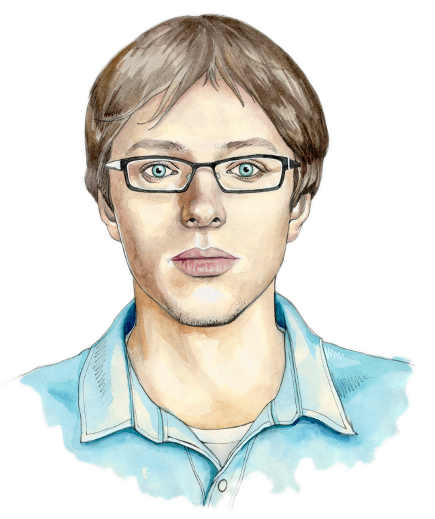
\includegraphics[width=5.5cm]{Photo.png}
\end{minipage}%
\hfill%
\begin{minipage}{0.6\textwidth}
\setstretch{1.0}
{\large\bf Eugene Burmako}\\
PhD, Computer Science\\
+1-631-464-1469\\
\href{mailto:eugene.burmako@gmail.com}{eugene.burmako@gmail.com}\\
San Francisco, CA\\
US Permanent Resident\\
\end{minipage}

\begin{resume}

\section{EXPERTISE}

Compilers,\\
Programming languages,\\
Developer tools.

\section{HIGHLIGHTS}

Cofounded and championed Swift MLIR, a toolchain that compiles ML programs written
in Swift into MLIR. Building on top of frontend metaprogramming via Swift quasiquotes
and backend metaprogramming via Swift Intermediate Language, we delivered
two prototypes that can compile small computational kernels and machine learning
models written in Swift to a combination of standard and XLA HLO dialects of MLIR.

Created Rsc, an experimental Scala compiler focused on compilation speed. Through outlining - really
quick computation of type signatures - we've been able to extract additional parallelism from Scala
builds and obtain significant compilation speedups. On Twitter Util, one of the foundational
libraries of the Twitter stack, our compilation pipeline is $\sim$2.7 times faster than the
traditional compilation pipeline on powerful hardware.

Cofounded and spearheaded Scalameta, an opensource toolchain that raises the bar of what is possible
for effective Scala development environment. Together with Denys Shabalin and \'{O}lafur P\'{a}ll
Geirsson, we turned Scalameta into a strategically important community initiative, which nowadays
encompasses more than 10 projects that add up to more than 13000 commits made by more than 200
contributors.
% Statistics obtained via `git rev-list --all --count` and `git shortlog -s -n`.

Designed and implemented reflection and macros for Scala together with Martin Odersky,
enabling a number of new patterns used in popular community libraries:
Akka, Play, Sbt, Scala.js, ScalaTest, Shapeless, Slick, Spark, Spire and others.

Bootstrapped the Scala macros community from zero to self-sustaining, gave more than 20 talks about
metaprogramming, managed more than 10 successful student projects, supervised the work of more than
40 contributors, provided help with more than 30 opensource projects.

Contributed $\sim$750 commits, $\sim$750 tests and $\sim$150k lines of code to the Scala compiler,
fixed $\sim$350 issues, being the 2nd top contributor to the Scala 2.10 release
and the 3rd top contributor to the Scala 2.11 release.

\section{PROJECTS}

\textbf{\href{http://go/swift-mlir}{Swift MLIR}}. Having learned about MLIR,
I've been looking for opportunities to integrate it into Swift, and in May 2019,
I found a plausible plan of attack and proceeded to work on what has become two
distinct prototypes - one based on Swift quasiquotes and another one based on Swift
Intermediate Language.

\begin{itemize} \itemsep -2pt
\item Proposed a design and a roadmap for integration between Swift and MLIR,
broke it down into bite-sized work items, evolved as necessary to adjust for
intermediate research findings and changes in the MLIR landscape.
\item Together with Alex Suhan, worked on the first prototype of Swift MLIR,
splitting the work between frontend (mostly myself) and backend (mostly Alex).
\item Explored lightweight modular staging, implemented virtualized if and for,
inspired by Scala virtualized, in the Swift compiler.
\item Implemented quasiquotes for the majority of Swift expressions
($\sim$2kloc compiler patch, $\sim$3kloc libQuote library, $\sim$3kloc libQuote tests).
\item Together with Adam Paszke, kickstarted libSIL - a Swift-based data model
and parser for Swift Intermediate Language.
\item Implemented the SIL dialect of MLIR and relevant components of a Swift
compilation pipeline that enable ingesting the intermediate representation of
the Swift compiler into the MLIR ecosystem.
\item Designed a prototype programming model and corresponding MLIR compiler
passes for the second prototype to compile small computational kernels and
machine learning models written in Swift to a combination of standard and
XLA HLO dialects of MLIR.
\end{itemize}

\textbf{\href{https://github.com/tensorflow/swift}{Swift for TensorFlow}}.
In Feb 2019, I joined the Swift for TensorFlow team at Google Brain to help build
a next-generation platform for machine learning founded by Chris Lattner et al.
During my time at the Swift for TensorFlow team, I was mostly focused on Swift MLIR,
but also made a few smaller contributions to Swift tooling and internal use cases
for our product.

\begin{itemize} \itemsep -2pt
\item Documented the state of internal tooling landscape for Swift for TensorFlow,
met with partner teams, proposed a roadmap for future work.
\item Investigated compilation performance of Swift for TensorFlow targets in
the Google monorepo, identified and documented areas of improvement.
\item Performed the initial investigation into SourceKit, implemented an MVP of
resolving cross-target references in the Google monorepo.
\item Figured out and documented how to enable Python interop and TPU support in
Swift for TensorFlow targets in the Google monorepo.
\end{itemize}

\textbf{\href{https://github.com/twitter/rsc}{Rsc}}. In Aug 2017, I started developing Rsc,
an experimental Scala compiler focused on compilation speed. Shortly after its inception,
the project got internal funding at Twitter. At the moment, Rsc is focused on outlining - really
quick computation of type signatures for an almost full subset of Scala. Once outlines are computed,
it becomes possible to compile all files of the program in parallel, which leads to significant
speedups on powerful hardware.

\begin{itemize} \itemsep -2pt
\item Owned internal and external roadmaps of Rsc, ensuring continuous delivery
on commitments in the face of significant uncertainty.
\item Worked together with partners within Advanced Scala Tools and Build teams towards
integration of Rsc into the Twitter toolchain and developer workflow.
\item Co-designed and implemented Rsc outlining, achieving significant coverage of Twitter internal
codebase.
\item Co-designed and prototyped RscCompat, an automated code rewrite that transforms Scala code
into a subset of Scala supported by Rsc.
\item Put together Warp - a simplistic build tool specialized for experiments with Rsc-based
toolchains.
\end{itemize}

\textbf{\href{http://scalameta.org/}{Scalameta}}. Based on the success of scala.reflect and
learning from user feedback, in Oct 2013 I set out to build a new metaprogramming platform for
Scala. Together with my colleague Denys Shabalin, we've laid out the axioms: 1) user convenience
comes first, 2) never lose a token or irreversibly desugar a tree, 3) always save typed ASTs into
the resulting bytecode. After my colleague \'{O}lafur P\'{a}ll Geirsson joined the project, we
shifted focus to developer tools which significantly increased the popularity of Scalameta.

\begin{itemize} \itemsep -2pt
\item Co-designed and implemented lexical, syntactic and semantic models for the Scala programming
language, tested them out in practice using the experience of working on the Scala compiler.
\item Co-designed and prototyped other aspects of the Scalameta vision (lightweight and portable
reflection API, quasiquoting and hygiene, AST interpreter, AST persistence, integration with build
tools, IDEs, etc).
\item Worked together with tool developers from the community to make sure that the new
metaprogramming platform adequately addresses their needs.
\item Evangelized and applied the research behind Scalameta in an industrial setting by designing
and building next-generation developer tools at Twitter.
\item Planned and managed the timeline of the project, organized opensource contributors
and their contributions.
\end{itemize}

\textbf{\href{https://github.com/scala/scala}{Scala}} is a statically-typed object-functional
programming language. Since Sep 2011, I'm a committer to scalac, the official Scala compiler.
During my first two years, I was a very active contributor to the compiler before moving my research
into separate repositories.

\begin{itemize} \itemsep -2pt
\item Contributed and maintained a novel language feature: def macros, along with the underlying
metaprogramming API.
\item Implemented Macro Paradise, a popular compiler plugin with additional macro flavors, which
was clocking 20k+ monthly downloads and ultimately got merged into the official Scala compiler.
\item Discovered and codified new tricks and idioms on the intersection of macros and vanilla Scala
features together with prominent community members.
\item Worked together with tool developers to enable support for the newly introduced language
features and patterns.
\item Fixed hundreds of issues in scalac, patching various subsystems of the compiler including
the parser and the typechecker.
\end{itemize}

\textbf{\href{http://scalamacros.org/}{Scala Macros}}. After joining the PhD program at EPFL in
Sep 2011, I've come up with an idea to implement macros in Scala. I realized the initial vision in
the official Scala compiler under the supervision of Martin Odersky and then proceeded to research
and preach new flavors of macros, gradually gaining support in the community. Very soon, macros
spread like wildfire, and now they are used in many popular libraries, including major components
of the Lightbend platform.

\begin{itemize} \itemsep -2pt
\item Co-designed and implemented scala.reflect, the library that has become the foundation for
compile-time and runtime metaprogramming in Scala 2.10.
\item Co-designed and implemented def macros for Scala 2.10.
\item Designed and realized a number of other macro flavors (dynamic macros, interpolation macros,
implicit macros, fundep materializers, type macros, type providers and macro annotations).
\item Promoted, documented and maintained Scala macros, communicating with the adopters
and contributors from the Scala community.
\item Provided consulting and support for a number of production and research users,
ramping up adoption of the new technologies.
\end{itemize}

\textbf{\href{https://github.com/scala/pickling}{Pickling}} is an experimental persistence library
for Scala that uses implicits and macros to derive extremely fast and customizable serializers,
matching and surpassing the performance of similar Java libraries. Pickling has gained popularity
and was eventually included in sbt, the most popular build tool for Scala.

\begin{itemize} \itemsep -2pt
\item Co-designed object-oriented pickler combinators.
\item Implemented and optimized the initial version of compile-time pickler generation facilities
that stood the test of time for more than two years.
\end{itemize}

\textbf{\href{http://code.google.com/p/conflux/}{Conflux}} is an experimental parallel programming
platform for C\# that I developed in 2010-2011. Conflux features a domain-specific language and
a high-level programming model that transparently distributes computational algorithms to GPUs both
in single-machine and cluster environments:

\begin{itemize} \itemsep -2pt
\item Designed and developed a high-level programming model in the form of an embedded DSL for C\#.
\item Implemented a C\# frontend: a C\# AST and a decompiler library.
\item Implemented a CUDA backend: a code generator for the PTX assembler of NVIDIA graphics processors
and a JIT compilation library.
\item Implemented a CPU backend: a code generator for multicore CPUs.
\item Provided integration with the Visual Studio debugger.
\end{itemize}

\textbf{\href{http://code.google.com/p/relinq/}{Relinq}} is a library for transforming C\#
expression trees into JavaScript code and vice versa. Relinq can be used to implement such scenarios
as: querying LINQ data sources from JavaScript, invoking cross-process LINQ queries and constructing
LINQ queries dynamically.

\begin{itemize} \itemsep -2pt
\item Designed and developed a JavaScript-based query language.
\item Extracted and documented a coherent subset of the C\# 3.0 specification.
\item Implemented an expression compiler for the aforementioned subset of C\# that supports generics,
lambdas and local type inference.
\end{itemize}

\textbf{\href{http://code.google.com/p/truesight-lite/}{Truesight}} is an experimental decompiler
for the bytecode of the .NET virtual machine. The library provides intermediate representation for
both low-level (bytecode) and high-level (abstract syntax tree) views of code. Truesight supports
basic constructs of C\# and is capable of decompiling structured control flow: conditionals, loops,
and restricted gotos (i.e. returns, breaks and continues).

\begin{itemize} \itemsep -2pt
\item Implemented a parser for CIL that reifies the bytecode and preserves debug information.
\item Designed and documented an intermediate tree-based representation for decompiled C\# code.
\item Implemented visualization for the IR: graphviz dumps, integration with the Visual Studio debugger.
\item Created and implemented an algorithm for decompilation of structured programs.
\end{itemize}

\textbf{\href{http://code.google.com/p/elf4b/}{Tiller}} is a C\# software suite for designing and
generating WYSIWYG interactive reports. It features a programming language that can be used to
specify formulae and to script report generation process. The programming language comes with
a JIT compiler that speeds up execution:

\begin{itemize} \itemsep -2pt
\item Designed and developed a script language.
% \item Integrated the language with existing domain-specific libraries.
\item Implemented a JIT compiler for the language.
\item Implemented a thread-safe ZIP-based engine for storing report components.
\end{itemize}

\section{WORK}

\emph{Google}\\
Mountain View, CA \\
Staff Software Engineer, Tech Lead / Manager \\
% 1600 Amphitheatre Parkway, Mountain View, CA 94043, United States of America
Feb 2020 - present\\
% 18 Feb 2020 - present
Activities: Our project exists at the intersection of Machine Learning and hardware,
but is still under wraps so we can't share much more detail.

\emph{Google}\\
Mountain View, CA \\
Staff Software Engineer \\
% 1600 Amphitheatre Parkway, Mountain View, CA 94043, United States of America
Feb 2019 - Feb 2020\\
% 11 Feb 2019 - 17 Feb 2020
Activities: Working on Swift for TensorFlow - a new way to develop machine learning models which
gives the power of TensorFlow directly integrated into Swift.

\emph{Twitter}\\
San Francisco, CA \\
Staff Software Engineer, Tech Lead of the Advanced Scala Tools team \\
% 1355 Market Street Suite 900, San Francisco, CA 94103, United States of America
Nov 2016 - Feb 2019 \\
% 14 Nov 2016 - 7 Feb 2019
Activities: Worked on my opensource Scala projects including Rsc, Scalameta and others to make
Scala tooling better - both internally inside the company and publicly in the Scala community.

\emph{\'{E}cole Polytechnique F\'{e}d\'{e}rale de Lausanne} \\
Lausanne, Switzerland \\
% Route Cantonale, 1015 Lausanne, Switzerland \\
Doctoral Assistant \\
% 1 Sep 2011 - 30 Sep 2016 \\
Sep 2011 - Nov 2016 \\
Activities: Did a PhD at EPFL, on the academic side of the Scala programming language team.
Along with the opensource work on putting my research in practice into Scala, I was also writing
occasional papers and doing teaching for the faculty.

\emph{ScienceSoft} \\
Minsk, Belarus \\
% 2 Bedy Street, 220040 Minsk, Belarus \\
Software Engineer \\
% 19 Nov 2007 - Aug 2011 \\
Nov 2007 - Aug 2011 \\
Activities: Enterprise software development with C\# and a little bit of JavaScript,
with integration into Microsoft Office and Microsoft SharePoint.

\emph{Itransition} \\
Minsk, Belarus \\
% 1 Kulman Street, 220013 Minsk, Belarus \\
Software Engineer \\
Oct 2005 - Sep 2007 \\
Activities: Enterprise software development with C\#.

\emph{Omega Software} \\
Minsk, Belarus \\
% 29 V.Horuzhej Street, 220123 Minsk, Belarus \\
Software Engineer \\
Oct 2004 - Sep 2005 \\
Activities: Enterprise software development with C++.

\section{EDUCATION}

\emph{\'{E}cole Polytechnique F\'{e}d\'{e}rale de Lausanne} \\
Lausanne, Switzerland \\
Sep 2011 - Mar 2017 \\
Degree: PhD in Computer Science \\
Thesis: \href{https://infoscience.epfl.ch/record/226166}{Unification of Compile-Time and Runtime Metaprogramming in Scala} \\

\emph{United Institute of Informatics Problems} \\
Minsk, Belarus \\
Nov 2009 - Oct 2012 \\
Degree: Researcher in Computer Science \\

\emph{Belarusian State University} \\
Minsk, Belarus \\
Sep 2003 - Jun 2008 \\
Degree: Specialist in Computer science \\

\section{MEMBERSHIPS}

\begin{itemize} \itemsep -2pt
\item Scala Center Advisory Board (Mar 2018 - Feb 2019)
\item Scala Language Server Protocol Working Group (Feb 2018 - Feb 2019)
\item GPCE 2018 Program Committee (Feb 2018 - Oct 2018)
\item Scala Symposium 2017 Program Committee (Apr 2017 - Oct 2017)
\item GPCE 2017 Program Committee (Dec 2016 - Oct 2017)
\item Scala Improvement Process Committee (Aug 2016 - Feb 2019)
\end{itemize}

\section{TALKS}

\begin{enumerate} \itemsep -2pt
\item \href{https://www.meetup.com/Swift-for-TensorFlow/events/262262835/}{E. Burmako, A. Suhan ``Swift as syntactic sugar for MLIR'', Swift for TensorFlow meetup, San Francisco, September 9, 2019}
\item \href{https://docs.google.com/presentation/d/1cJQPJMTa7IJqCpJf4WpVM_UpiSivsmfnsMbBmodNh3M/edit#slide=id.g5dc464bf19_0_98}{E. Burmako, A. Suhan ``Swift as syntactic sugar for MLIR'', Google ML Languages Summit, San Francisco, August 13, 2019}
\item \href{https://docs.google.com/presentation/d/1WOR288YE4-qgjtPtnb7taK0KrhTFTfMf_e-Vvv29vbE/edit}{E. Burmako ``Swift for TensorFlow: A new way of doing machine learning'', Google Developers ML Summit, Tokyo, July 11, 2019}
\item \href{https://github.com/twitter/rsc/raw/master/docs/2018-11-15-ScaleByTheBay.pdf}{E. Burmako ``Towards Parallelizing Scala Compilations'', Scale by the Bay, San Francisco, November 15, 2018}
\item \href{https://2018.splashcon.org/track/meta-2018#About}{E. Burmako ``SemanticDB: a Common Data Model for Scala Developer Tools'', Workshop on Meta-Programming Techniques and Reflection, Boston, November 5, 2018}
\item \href{https://conf.researchr.org/track/scala-2018/scala-2018-papers#About}{E. Burmako ``SemanticDB: a Common Data Model for Scala Developer Tools'', Scala Symposium, September 28, 2018}
\item \href{http://scalameta.org/talks/2018-06-20-HowWeBuiltToolsThatScaleToMillionsOfLoc.pdf}{E. Burmako ``How We Built Tools That Scale to Millions of Lines of Code'', Scala Days, New York City, June 20, 2018}
\item \href{https://github.com/twitter/rsc/raw/master/docs/2017-11-16-ScaleByTheBay.pdf}{E. Burmako ``Reasonable Scala Compiler'', Scale by the Bay, San Francisco, November 16, 2017}
\item \href{http://scalamacros.org/paperstalks/2017-06-07-ConcreteNextSteps.pdf}{E. Burmako ``Concrete Next Steps for Scala Macros'', SF Scala, San Francisco, June 7, 2017}
\item \href{http://scalameta.org/talks/2017-06-01-SemanticToolingAtTwitter.pdf}{E. Burmako, S. Hood ``Semantic Tooling at Twitter'', Scala Days, Copenhagen, June 1, 2017}
\item \href{http://scalameta.org/talks/2017-06-01-SemanticToolingAtTwitter.pdf}{E. Burmako, S. Hood ``Semantic Tooling at Twitter'', Scala Days, Chicago, Apr 21, 2017}
\item \href{http://scalamacros.org/paperstalks/2017-03-02-ScalaSphere.pdf}{E. Burmako ``Scala.Meta Semantic API'', ScalaSphere DevTools Summit, Krak\'{o}w, Mar 2-3, 2017}
\item \href{http://scalamacros.org/paperstalks/2016-12-08-Scalax.pdf}{E. Burmako ``A New Macro System for Scala'', Scala eXchange, London, Dec 8, 2016}
\item \href{http://scalamacros.org/paperstalks/2016-11-12-ScalaByTheBay.pdf}{E. Burmako ``Scala.Meta: the Past, the Present and the Future'', Scala by the Bay, San Francisco, Nov 12, 2016}
\item \href{http://scalamacros.org/paperstalks/2016-07-19-ToMacrosAndBeyond.pdf}{E. Burmako ``To Macros and Beyond!: How macros changed Scala, and what's coming next'', Curry On, Rome, Jul 19, 2016}
\item \href{http://scalamacros.org/paperstalks/2016-06-17-Metaprogramming20.pdf}{E. Burmako ``Metaprogramming 2.0: No, Macros Are Not Going Away'', Scala Days, Berlin, Jun 17, 2016}
\item \href{http://scalamacros.org/paperstalks/2016-05-11-Metaprogramming20.pdf}{E. Burmako ``Metaprogramming 2.0'', Scala Days, New York City, May 11, 2016}
\item \href{http://scalamacros.org/paperstalks/2016-02-11-WhatDidWeLearnInScalaMeta.pdf}{E. Burmako ``What Did We Learn In Scala Meta?'', ScalaSphere DevTools Summit, Krak\'{o}w, Feb 11, 2016}
\item E. Burmako ``State of the Meta, Fall 2015'', fby.by, Minsk, Nov 28, 2015
\item \href{https://github.com/scalameta/tutorial}{E. Burmako ``Hands on Scala.Meta'', Scala World, Lake District, Sep 21, 2015}
\item \href{http://scalamacros.org/paperstalks/2015-06-09-StateOfTheMetaSummer2015.pdf}{E. Burmako ``State of the Meta, Summer 2015'', Scala Days, Amsterdam, Jun 09, 2015}
\item \href{http://scalamacros.org/paperstalks/2015-03-17-StateOfTheMetaSpring2015.pdf}{E. Burmako ``State of the Meta, Spring 2015'', Scala Days, San Francisco, Mar 17, 2015}
\item \href{http://scalamacros.org/paperstalks/2014-11-22-TheStateOfTheMeta.pdf}{E. Burmako ``State of the Meta, Fall 2014'', f(by) - Conference on Functional Programming, Minsk, Nov 22, 2014}
\item \href{http://scalamacros.org/paperstalks/2014-06-17-EasyMetaprogrammingForEveryone.pdf}{E. Burmako, D. Shabalin ``Easy Metaprogramming For Everyone!'', Scala Days, Berlin, Jun 16-18, 2014}
\item \href{https://github.com/scalamacros/macrology201}{E. Burmako, D. Shabalin ``Macrology 201'', flatMap, Oslo, May 12-13, 2014}
\item \href{https://github.com/travisbrown/type-provider-examples/blob/master/docs/scalar-2014-slides.pdf?raw=true}{E. Burmako, T. Brown ``Macro-Based Type Providers in Scala'', Scalar, Warsaw, Apr 5, 2014}
\item \href{http://scalamacros.org/paperstalks/2014-03-02-RethinkingScalaMacros.pdf}{E. Burmako ``Rethinking Scala Macros'', Northeast Scala Symposium, New York, March 1-2, 2014}
\item \href{http://scalamacros.org/paperstalks/2014-03-01-MacrosVsTypes.pdf}{E. Burmako, L. Hupel ``Macros vs Types'', NE Scala, New York, March 1-2, 2014}
\item \href{http://scalamacros.org/paperstalks/2014-02-04-WhatAreMacrosGoodFor.pdf}{E. Burmako ``What Are Macros Good For?'', Scala eXchange, London, December 2-3, 2013}
\item \href{http://scalamacros.org/paperstalks/2013-11-25-ScalaMacrosPoster.pdf}{E. Burmako, D. Shabalin ``Scala Macros'', Google PhD Student Summit on Compiler \& Programming Technology, Munich, November 25, 2013}
\item \href{http://scalamacros.org/paperstalks/2013-09-19-PhilosophyOfScalaMacros.pdf}{E. Burmako ``Philosophy of Scala Macros'', Strange Loop, St. Louis, September 18-19, 2013}
\item \href{http://scalamacros.org/paperstalks/2014-02-04-WhatAreMacrosGoodFor.pdf}{E. Burmako ``What Are Macros Good For?'', Scalape\~{n}o, Tel Aviv, July 17, 2013}
\item \href{http://scalamacros.org/paperstalks/2013-06-13-AppliedMaterialization.pdf}{E. Burmako ``Applied Materialization'', Bay Area Scala Enthusiasts, San Francisco, June 13, 2013}
\item \href{http://scalamacros.org/paperstalks/2013-06-12-HalfYearInMacroParadise.pdf}{E. Burmako ``Half a Year in Macro Paradise'', Scala Days, New York City, June 10-12, 2013}
\item \href{https://github.com/scalamacros/scalamacros.github.com/raw/master/paperstalks/2013-03-31-ScalaMacros.pdf}{E. Burmako ``Macros in Scala'', Codefest, Novosibirsk, March 30-31, 2013}
\item \href{https://github.com/scalamacros/scalamacros.github.com/raw/master/paperstalks/2012-04-28-MetaprogrammingInScala210.pdf}{E. Burmako ``Metaprogramming in Scala 2.10'', Minsk, April 28, 2012}
\item \href{https://github.com/scalamacros/scalamacros.github.com/raw/master/paperstalks/2012-04-18-ScalaDays2012.pdf}{E. Burmako, J. C. Vogt ``Scala Macros'', Scala Days, London, April 17-18, 2012}
\item \href{https://github.com/scalamacros/scalamacros.github.com/raw/master/paperstalks/2011-09-27-ProjectKepler.pdf}{E. Burmako ``Project Kepler: Compile-Time Metaprogramming for Scala'', Lausanne, September 27, 2011}
\item \href{https://code.google.com/archive/p/conflux/downloads}{E. Burmako ``Conflux: GPGPU for .NET'', 1st International Conference, Application Developer Days, Yaroslavl, 2010}
\item A. Varanovich, V. Tulchinsky, E. Burmako, V. Falfushinsky, R. Sadykhov ``Automated Software Development in Heterogeneous GPU/CPU Environments for Seismic Modeling'', EAGE, Barcelona, 2010
\end{enumerate}

\section{PAPERS}

\begin{enumerate} \itemsep -2pt
\item \href{https://infoscience.epfl.ch/record/226166}{E. Burmako, M. Odersky ``Unification of Compile-Time and Runtime Metaprogramming in Scala'', PhD thesis, Lausanne, March, 2017}
\item \href{https://infoscience.epfl.ch/record/200963}{V. Ureche, E. Burmako, M. Odersky ``Late Data Layout: Unifying Data Representation Transformations'', Object Oriented Programming Systems Languages \& Applications, Portland, October 19-21 2014}
\item \href{http://scalamacros.org/paperstalks/2014-07-29-MorphScala.pdf}{A. Biboudis, E. Burmako ``MorphScala: Safe Class Morphing with Macros'', Scala Workshop, Uppsala, Jul 28-29, 2014}
\item \href{http://infoscience.epfl.ch/record/187787}{H. Miller, P. Haller, E. Burmako, M. Odersky. ``Instant Pickles: Generating Object-Oriented Pickler Combinators for Fast and Extensible Serialization'', Object-Oriented Programming, Systems, Languages \& Applications, Indianapolis, October 26-31, 2013}
\item \href{https://infoscience.epfl.ch/record/186844}{E. Burmako ``Scala Macros: Let Our Powers Combine!'', Scala Workshop, Montpellier, July 2, 2013}
\item \href{https://infoscience.epfl.ch/record/185242}{D. Shabalin, E. Burmako, M. Odersky ``Quasiquotes for Scala'', Technical report, Lausanne, March, 2013}
\item \href{http://infoscience.epfl.ch/record/183862}{E. Burmako, M. Odersky ``Scala Macros'', Valentin Turchin Workshop on Metacomputation, Pereslavl-Zalessky, July 5-9, 2012}
\item \href{https://code.google.com/archive/p/conflux/downloads}{E. Burmako, R. Sadykhov ``Conflux: Embedding Massively Parallel Semantics in a High-Level Programming Language'', Pattern Recognition and Information Processing, Minsk, 2011}
\item E. Burmako, R. Sadykhov ``Compilation of high-level programming languages for execution on graphical processor units'', Supercomputer Systems and Applications, Minsk, 2010
\item A. Varanovich, E. Burmako, R. Sadykhov ``Implementation of CUDA kernels for execution in multiprocessor systems with the use of dynamic runtime'', Technologies of high-performance computing and computer-aided modeling, St. Petersburg, 2010
\end{enumerate}

\end{resume}
\end{document}
